\documentclass[letterpaper]{article}

\usepackage{natbib,alifeconf}  %% The order is important

\usepackage{hyperref}

% *****************
%  Requirements:
% *****************
%
% - All pages sized consistently at 8.5 x 11 inches (US letter size).
% - PDF length <= 8 pages for full papers, <=2 pages for extended
%    abstracts.
% - Abstract length <= 250 words.
% - No visible crop marks.
% - Images at no greater than 300 dpi, scaled at 100%.
% - Embedded open type fonts only.
% - All layers flattened.
% - No attachments.
% - All desired links active in the files.

% Note that the PDF file must not exceed 5 MB if it is to be indexed
% by Google Scholar. Additional information about Google Scholar
% can be found here:
% http://www.google.com/intl/en/scholar/inclusion.html.


% If your system does not generate letter format documents by default,
% you can use the following workflow:
% latex example
% bibtex example
% latex example ; latex example
% dvips -o example.ps -t letterSize example.dvi
% ps2pdf example.ps example.pdf


% For pdflatex users:
% The alifeconf style file loads the "graphicx" package, and
% this may lead some users of pdflatex to experience problems.
% These can be fixed by editing the alifeconf.sty file to specify:
% \usepackage[pdftex]{graphicx}
%   instead of
% \usepackage{graphicx}.
% The PDF output generated by pdflatex should match the required
% specifications and obviously the dvips and ps2pdf steps become
% unnecessary.


% Note:  Some laser printers have a serious problem printing TeX
% output. The use of ps type I fonts should avoid this problem.

\title{Multi-modeling the morphogenesis of transportation networks}
\author{Juste Raimbault$^{1,2}$\\
\mbox{}\\
$^1$UPS CNRS 3611 ISC-PIF, Paris, France \\
$^2$UMR CNRS 8504 G{\'e}ographie-cit{\'e}s, Paris, France \\
juste.raimbault@polytechnique.edu} % email of corresponding author

% For several authors from the same institution use the same number to
% refer to one address.
%
% If the names do not fit well on one line use
%         Author 1, Author 2 ... \\ {\Large\bf Author n} ...\\ ...
%
% If the title and author information do not fit in the area
% allocated, place \setlength\titlebox{<new height>} after the
% \documentclass line where <new height> is 2.25in



\begin{document}
\maketitle

\begin{abstract}
% Abstract length should not exceed 250 words
This research introduces a multi-modeling approach to the growth of transportation networks. More precisely, we implement and compare several models, based on biological network growth, cost-benefit rules, and gravity potential breakdown. The resulting multi-modeling framework is calibrated on observed topological data for the European road network. We show that different heuristics are complementary to cover the feasible topological space and that all are necessary to approach existing configurations, what suggests the superposition of corresponding processes in territorial systems.
\end{abstract}

% keywords : network morphogenesis, multi-modeling, territorial systems

%\section{Introduction}

The growth of transportation networks in territorial systems bears stunning similarities with biological networks, and the understanding of processes driving their spatial extension can both have practical planning applications but also bring theoretical insights into complex morphogenetic systems. Network growth models have been proposed in several disciplines, of which \cite{xie2009modeling} give a large overview, taking into account diverse processes such as economical, geometrical, geographical processes for example. There exists to our knowledge no systematic comparison of different network generation heuristics. We develop here such a comparison in a multi-modeling paradigm.


\section{Modeling network growth}

We introduce a general model of road network growth, conditioned to a fixed population density on a grid, in a sequential way with the following steps. A common core ensures the positioning of new centers preferentially to population density and a direct connection to the existing network. Nodes and links are then added following different potential processes corresponding to the selected heuristic: (i) no supplementary growth (baseline); (ii) random links; (iii) biological network growth following the model of \cite{tero2010rules}, where new links are taken as the links with the highest capacity in the stationary flow network obtained by evolving capacities of the full network of potential new links; (iv) cost-benefit network growth as proposed by \cite{louf2013emergence}; (v) stochastic gravity potential breakdown as used by \cite{schmitt2014modelisation}; and (vi) a novel model based on thresholded deterministic potential breakdown. The network is grown until reaching a fixed number of new nodes to ensure comparability between the different heuristics.

A network is then quantified by topological indicators, namely average closeness and betweenness centralities, diameter, efficiency, and average path length. To compare the generated network to real data, we collected the European street network from the open data provided by OpenStreetMap, and extracted the value of topological indicators on 50km side moving windows. Typical configurations were then selected according to morphological classes for population density. The corresponding real network measures are compared to network generated on the same population density configurations, for 50 different configurations.



\begin{figure*}[h!]
\vspace{-0.5cm}
\begin{minipage}[c]{0.45\linewidth}
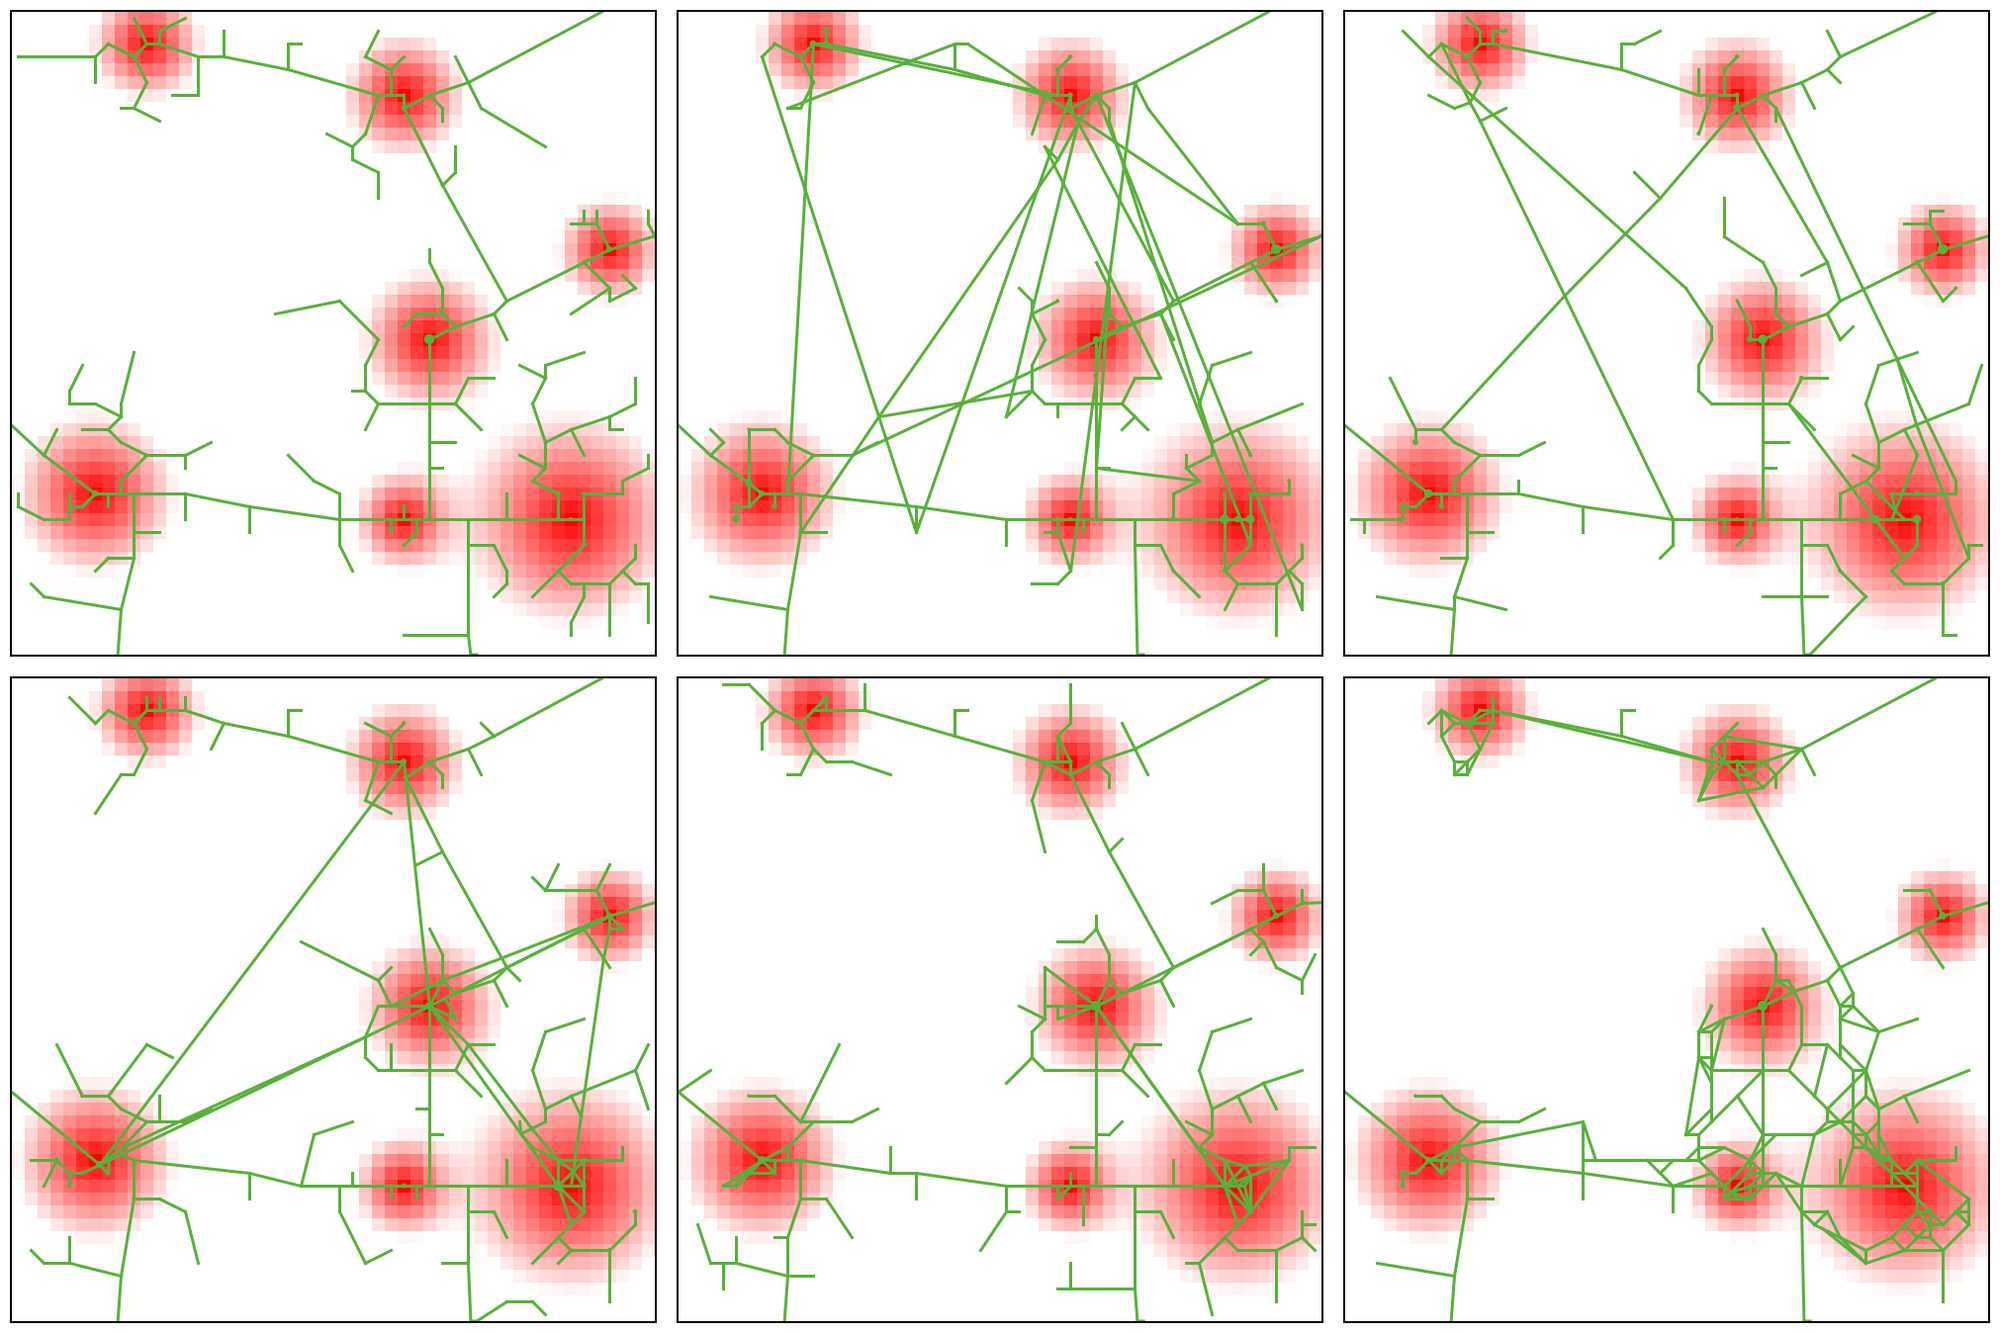
\includegraphics[width=\linewidth]{figures/7-1-2-fig-networkgrowth-examples.jpg}\\
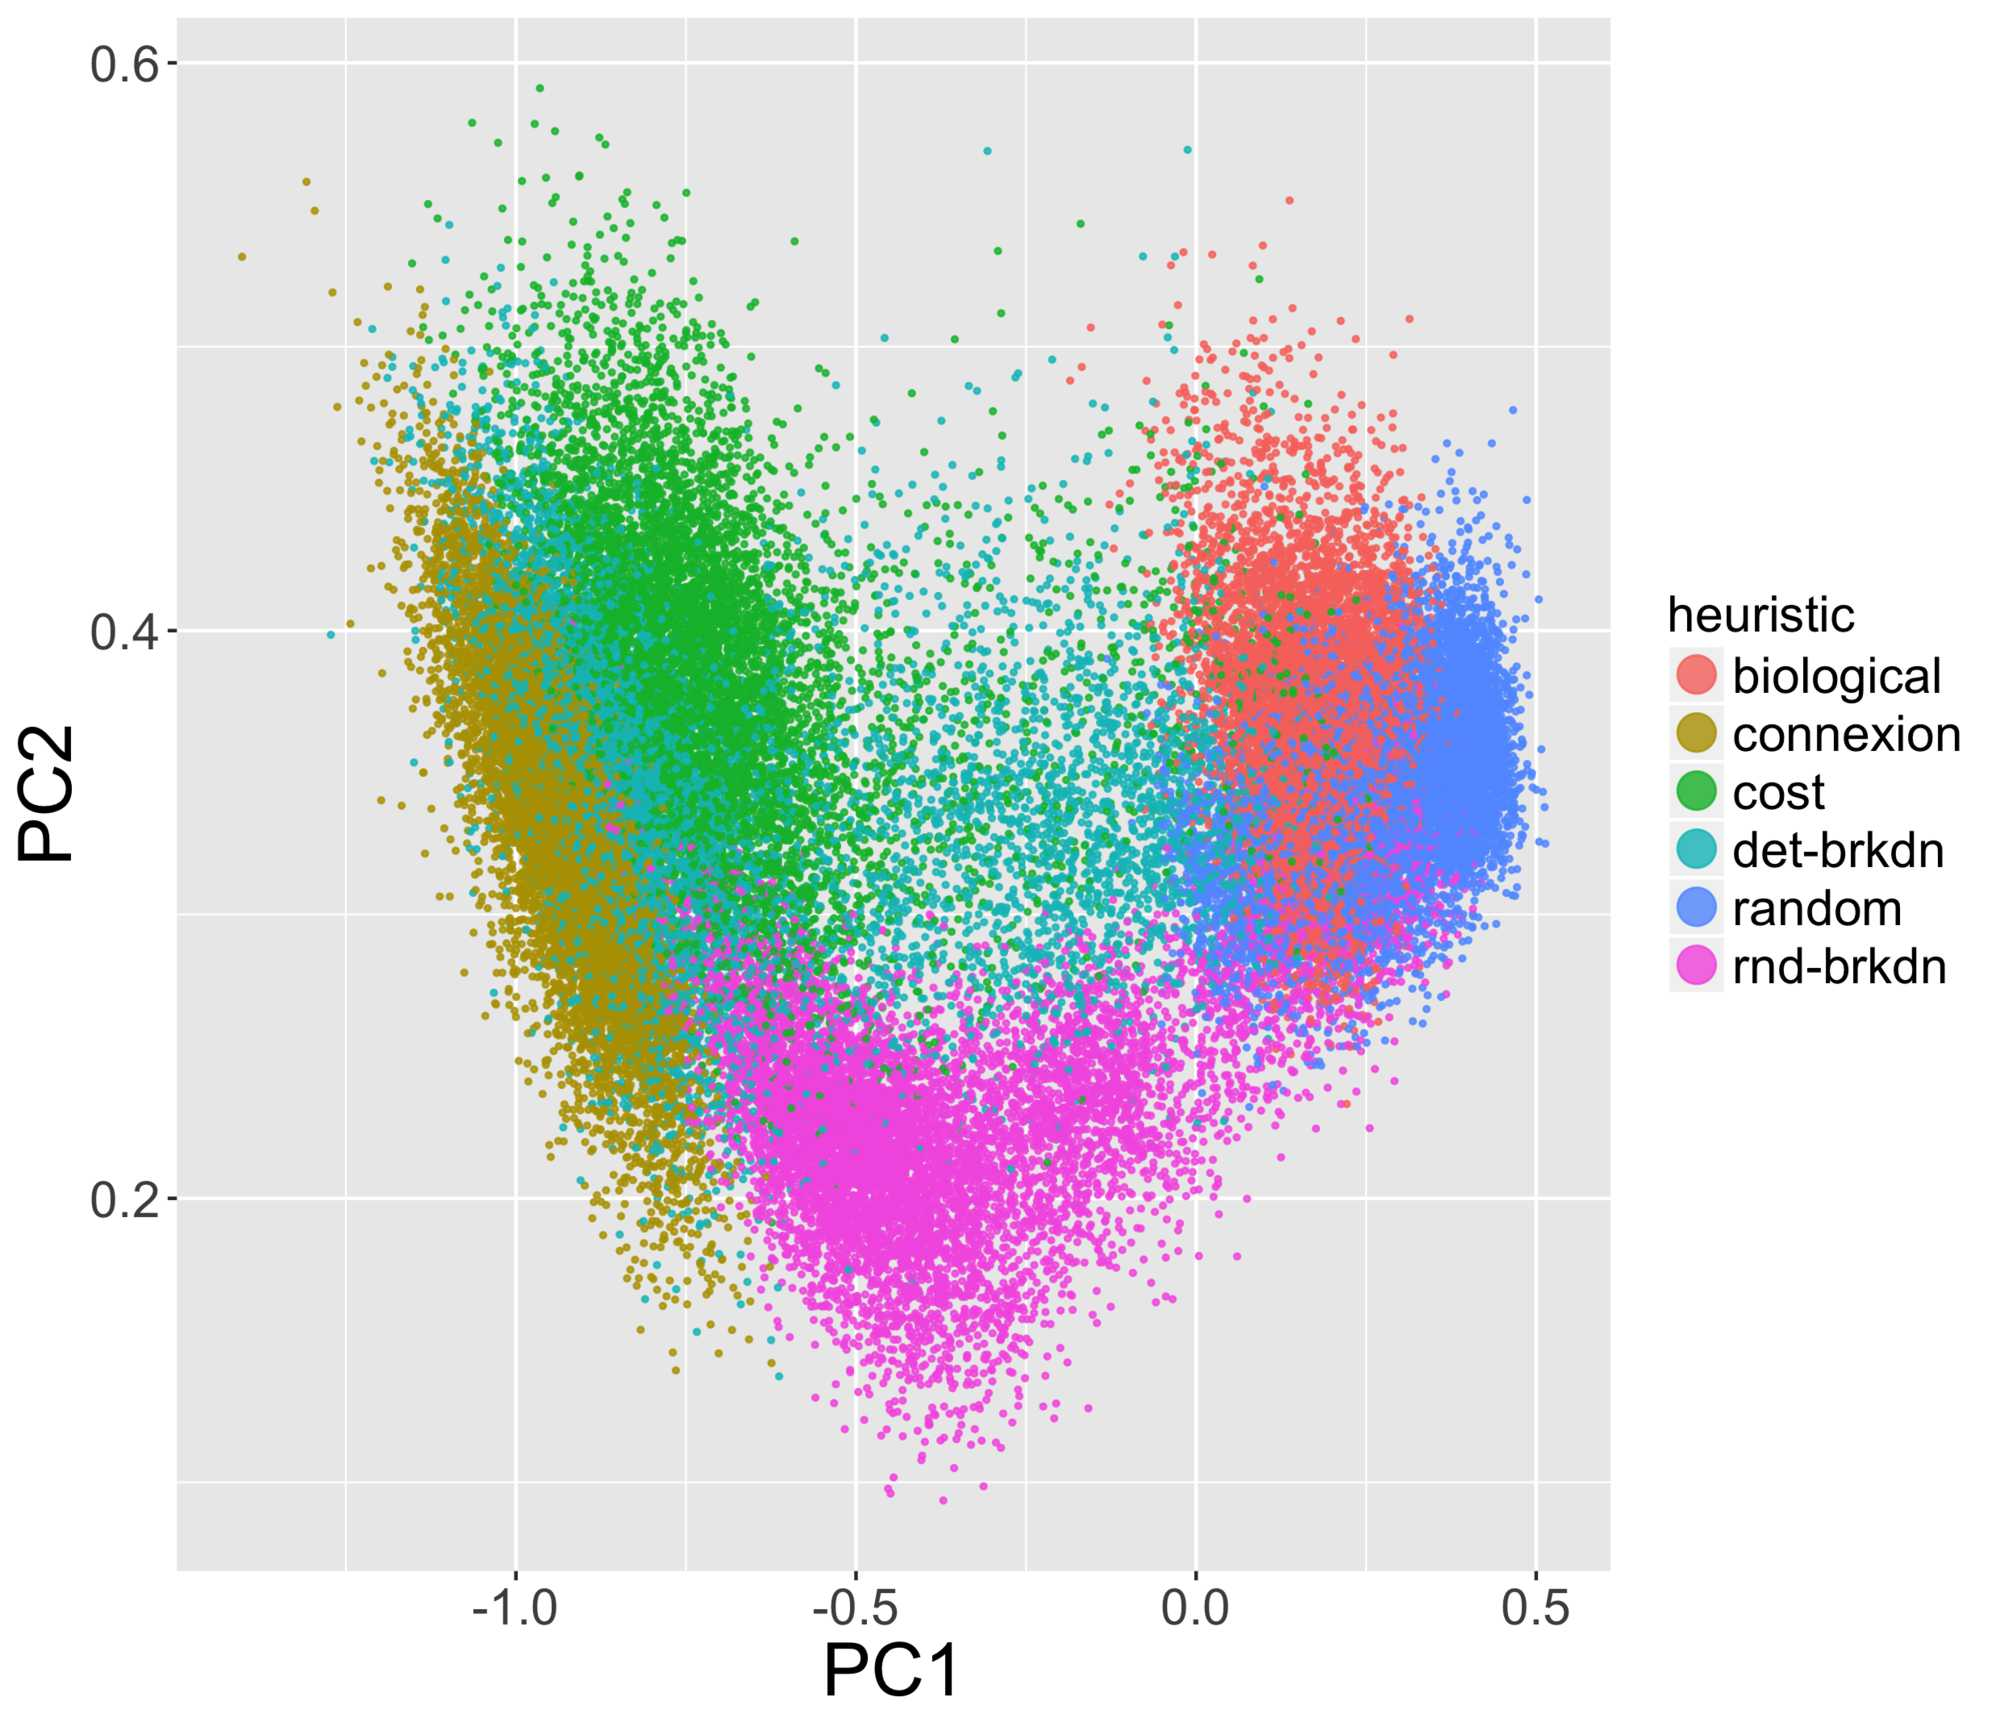
\includegraphics[width=\linewidth]{figures/7-1-2-fig-networkgrowth-feasiblespace.jpg}\\
\end{minipage}
\begin{minipage}[c]{0.55\linewidth}
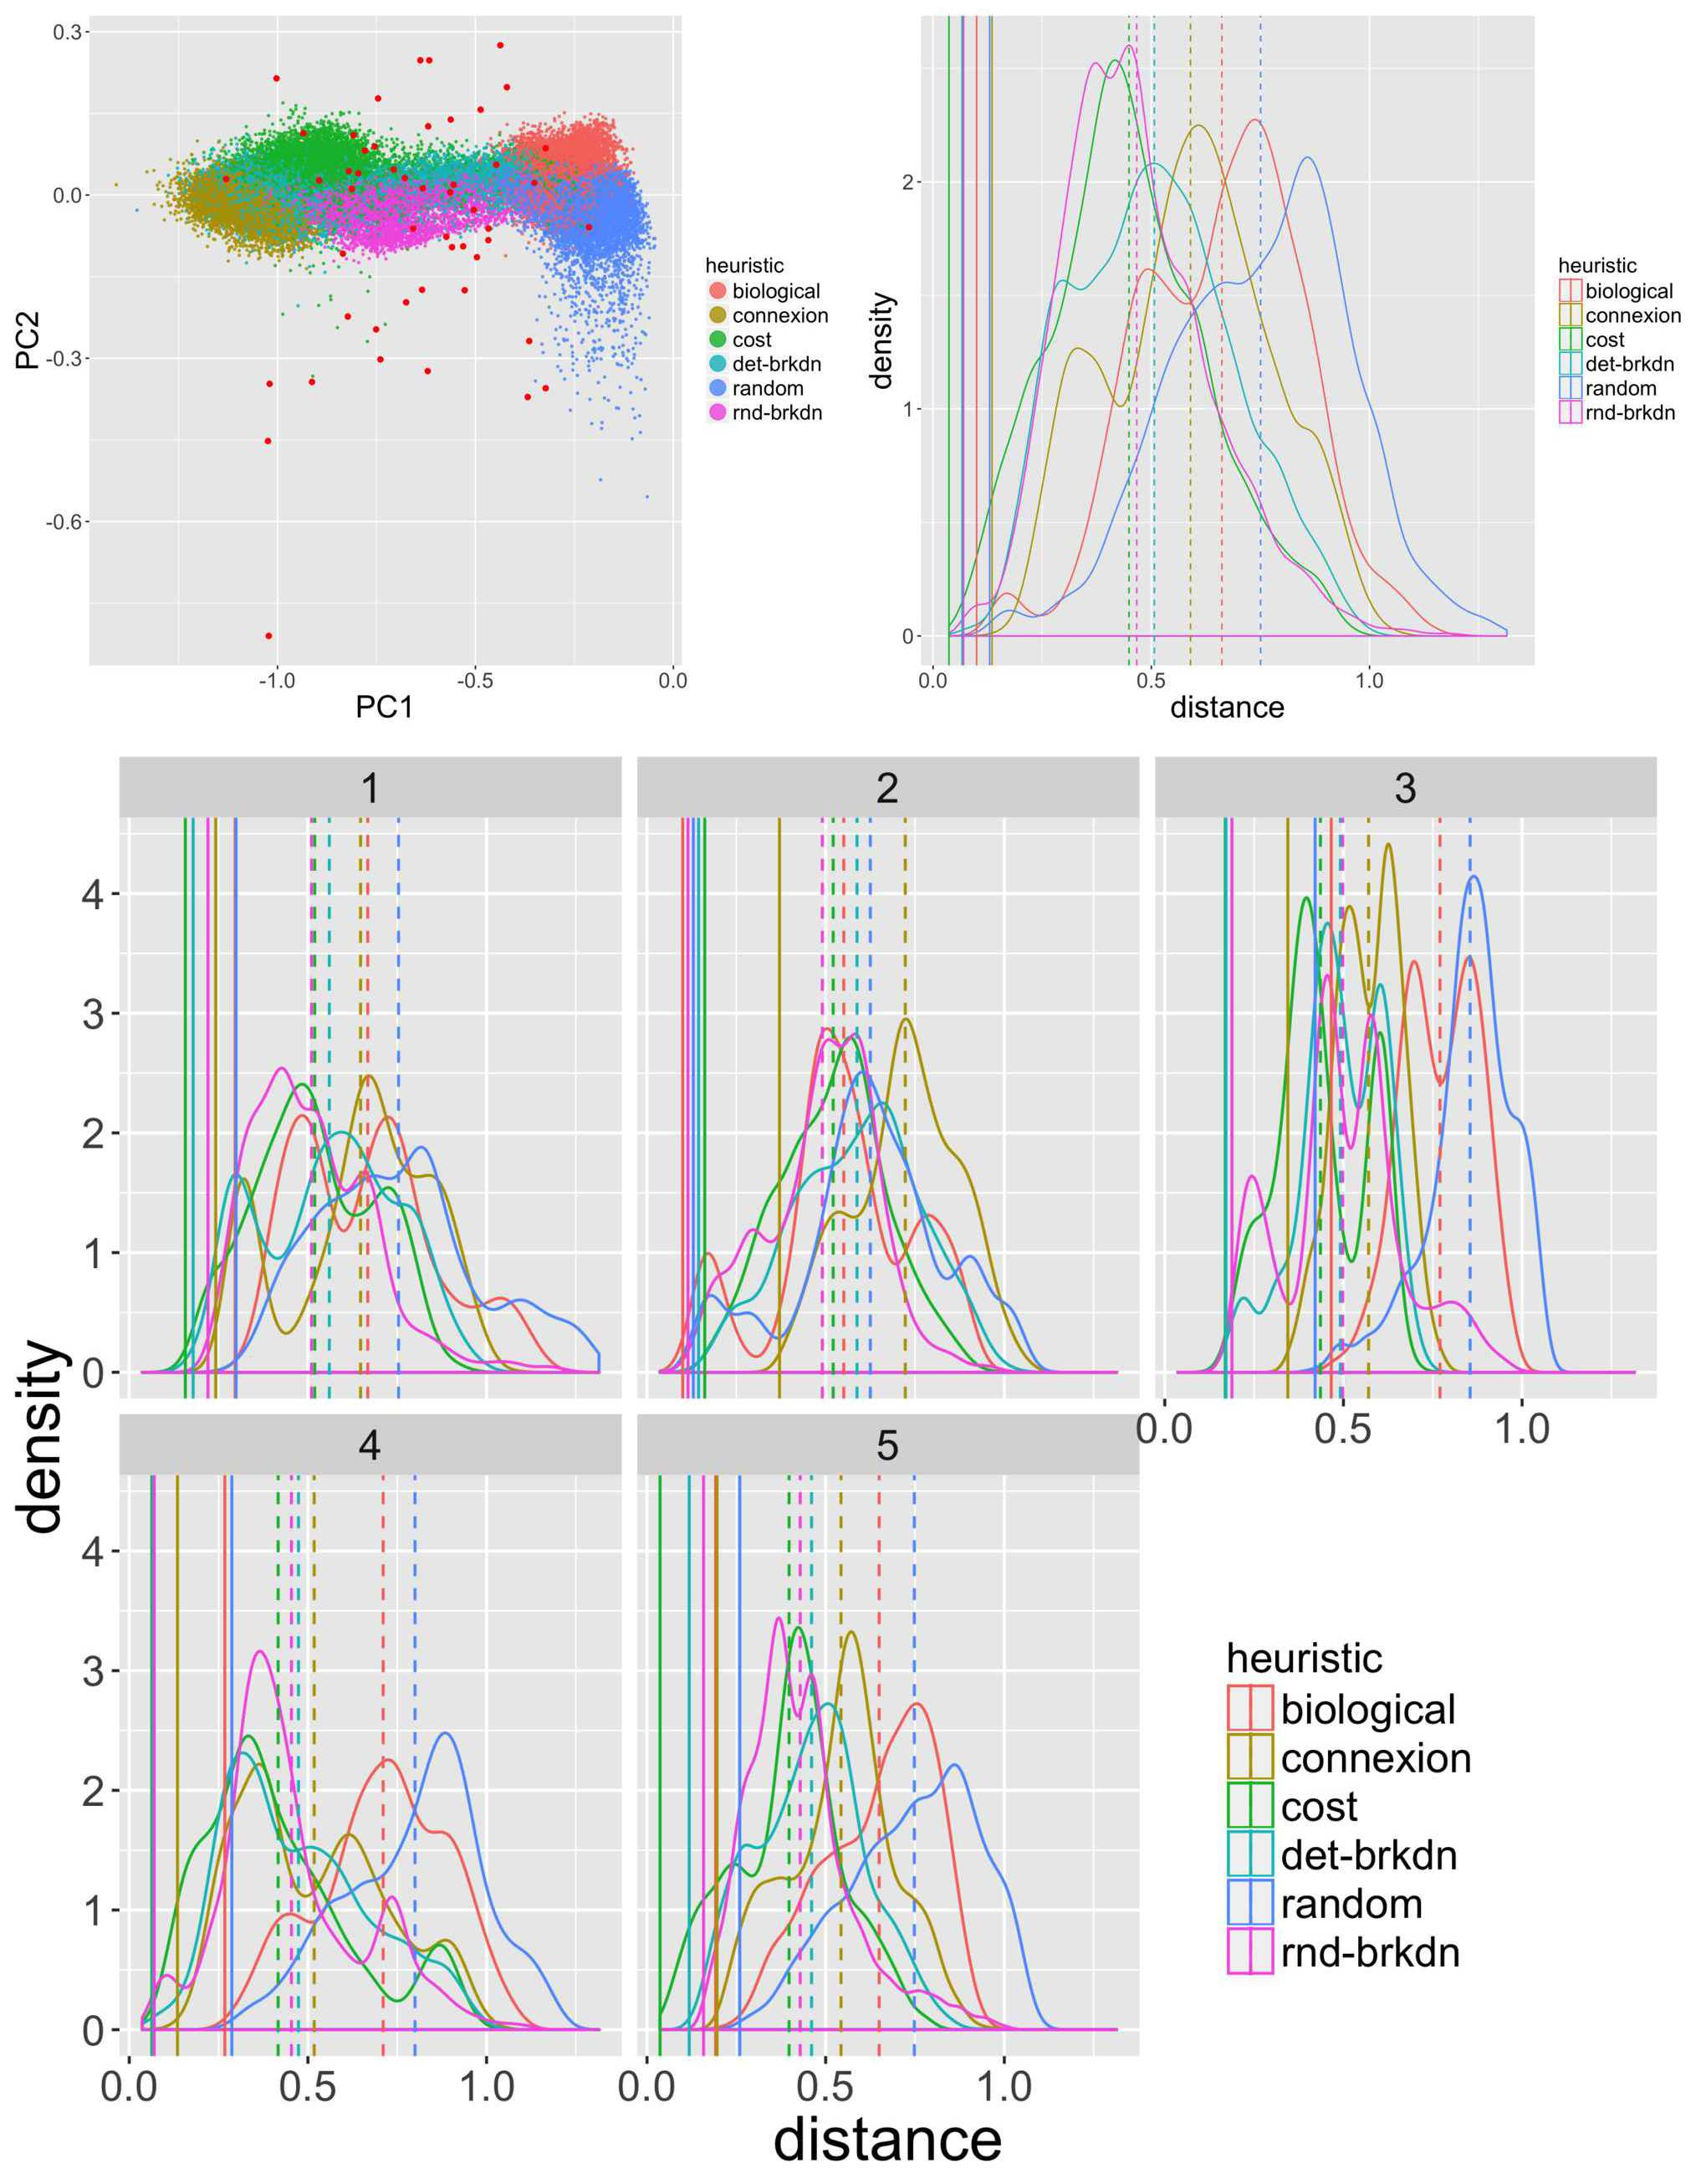
\includegraphics[width=\linewidth]{figures/7-1-2-fig-networkgrowth-realdistance.jpg}
\end{minipage}
\caption{\textit{(Top left)} Examples of network configuration generated by the different heuristics; \textit{(Bottom Left)} Feasible space of topological indicators for networks generated by the model, shown in a reduced dimension after principal component analysis, with a different color for each heuristic; \textit{(Right)} Feasible space with red points corresponding to real networks, and histograms of indicator distance to data, for all densities configuration and conditioned by the type of urban form.}
\label{fig:fig1}
\end{figure*}

\section{Results}

The heterogeneity of models suggested the choice of an implementation in NetLogo which handles easily heterogenous multi-agent systems. Source code and results are available on the open repository of the project\footnote{at \url{https://github.com/JusteRaimbault/CityNetwork/tree/master/Models/MesoCoevol}}. The parameter space of the model is explored using the workflow engine OpenMOLE \citep{reuillon2013openmole} which allows an easy distribution of tasks on a computation grid.


We sample for each density configuration 1000 parameter points (including the generation heuristic and specific parameters for each heuristic in the random LHS sampling) and repeat the stochastic model 5 times for each point. Results are shown in Fig.~\ref{fig:fig1} below. We illustrate for a synthetic population density configuration the different types of networks obtained. The feasible space covered by the sampling in the reduced indicator space (two first components of a principal component analysis) is such that heuristics are complementary to cover the full area, and overlap between point clouds quantified with a concentration index are low (Herfindhal index with a first quartile at 0.54 on a grid of size 20 separating the reduced indicator space). This complementarity is confirmed when comparing to the indicator values for real networks: some points fall relatively far from the point cloud, but each heuristic captures some real configurations. The distribution of distances of simulated points to real points confirm this low minimum for each heuristic. When conditioned by morphological class for population density, we obtain varying behavior regarding the most performant heuristic, conforming that different urban regimes are associated to specific network morphogenesis processes.

Therefore, our work demonstrates that, among the heuristic we compared, there is no best model to reproduce real configurations and that all processes included are complementary. Possible developments include a more refined calibration to find for typical configurations of real networks the heuristic and parameters producing the closest networks, or a comparison between heuristics controlling for the number of parameters to take overfitting into account (which could be here at the origin of the low performance of the biological heuristic e.g.). We also suggest that similar benchmarks should be more systematically performed for the modeling of complex territorial systems.
%, to pave the way towards more complex models progressively coupling existing complementary perspectives.



%\section{Discussion}







\footnotesize
\bibliographystyle{apalike}
\bibliography{biblio} % replace by the name of your .bib file


\end{document}
